\chapter{Bevezetés} % Introduction
\label{ch:intro}

Ha valaki játékfejlesztésbe szeretne kezdeni, akkor nagyon sok kihívással kell szembenéznie. Szerencsére manapság már levehet egy terhet a válláról ha egy előre megírt játékmotort (\textbf{game engine}) használ, amiből akár ingyenesen elérhetőt is lehet találni.

Egy játékmotor feladata hogy leegyszerűsítse a kirajzolást és az objektumok \textbf{valósághű viselkedését}. Ilyen viselkedés például, ha két szilárd tárgy ütközésekor azt várnánk el hogy azok ne menjenek bele egymásba, hanem inkább ténylegesen ütközzenek és akár pattanjanak le a másikról. Ezen viselkedés kiszámolása meglehetősen költséges tud lenni, ráadásul különböző alakzatoknál különböző algoritmusokat kell használni.

Szakdolgozatomban azzal foglalkozom hogy hogyan lehet a kirajzolást és az előbb említett valósághű viselkedést fraktálokkal elvégezni. A velük való ütközéshez megállapításához ugyanaz fog segítséget nyújtani, mint a kirajzolásukhoz: távolságfüggvények. 


\begin{figure}[H]
	\centering
	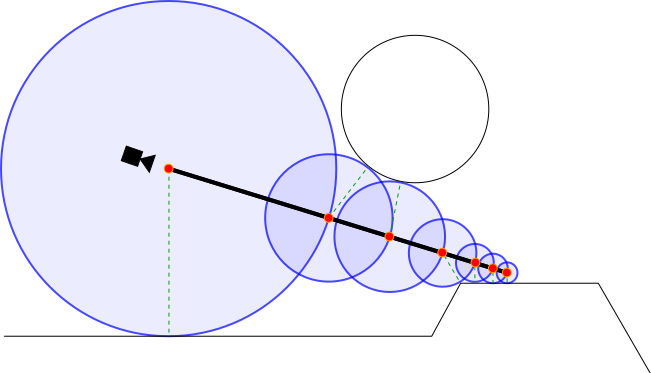
\includegraphics[width=0.4\textwidth]{SphereTracing}
	\caption{Sphere tracing: A kamerából kiinduló fénysugár mindig csak annyit halad előre amekkora a hozzá legközelebb lévő felület távolsága \cite{Raymarch94:online}}
	\label{fig:SphereTracing}
\end{figure}

Hogyan valósítom ezt meg? A kirajzoláshoz \textbf{Sphere tracing} módszert (\ref{fig:SphereTracing}. ábra) alkalmazok, így minden kirajzolt objektumomhoz van távolságfüggvényem. Ezek segítségével meg tudom állapítani a virtuális terem bármely pontjáról hogy az milyen messze van a kirajzolt felületektől. 

Ezen tudással nagyon egyszerűen és hatékonyan meg lehet állapítani hogy egy gömb ütközött-e bármivel, hiszen csak annyit kell ellenőriznünk hogy a gömb középpontja gömbsugárnyi távolságra van-e valamilyen felülettől. Ezután már csak meg kell határoznunk hogy mit tegyen a gömb ütközés esetén, amihez jó kiindulási alap ha a felületről visszaverődő fénysugárként tekintünk rá -- mivel annak kiszámolására jól ismert algoritmus van.

\begin{figure}[H]
	\centering
	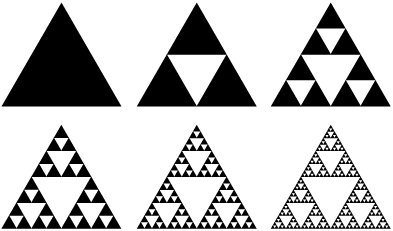
\includegraphics[width=0.6\textwidth]{haromszog}
	\caption{Példa egy IFS-re: a Sierpiński háromszög néhány iterációja \cite{Sierpins37:online}}
	\label{fig:Ifs}
\end{figure}

Ezen megközelítéshez azonban pontos és lehetőleg előjeles távolságfüggvények kellenek, így esetünkben nem érdemes foglalkozni az olyan fraktálokkal amikhez a távolságfüggvény csak felső becslést ad. 

Ezért a fraktálok egy olyan csoportjával foglalkozom, mint a Sierpiński háromszög (\ref{fig:Ifs}. ábra), amik \textbf{IFS (Iterated Function System)}  által jönnek létre, azaz egy egyszerűbb alakzaton -- aminek jól ismerjük a pontos távolságfüggvényét -- sokszor végrehajtunk egymás után transzformációkat. Az ilyen fraktálokat könnyű generálni, mert ha eldöntöttük milyen transzformációink lesznek, azok újraparaméterezésével könnyen meghatározhatunk egy újabb fraktált leíró távolságfüggvényt.
